In this paper, we consider the problem of using mobile robots equipped 
with range sensors to guard (1D) perimeters or (2D) regions. Given 
a bounded polygonal one- or two-dimensional set to be secured, 
and $k$ mobile robots where robot $i$'s sensor covers a circular region of 
radius $r_i$, we seek a deployment of the robots so that $\max r_i$ is 
minimized. That is, we would like to minimize the maximum single-sensor 
coverage across all sensors. We denote this multi-sensor coverage problem 
under the umbrella term {\em optimal set guarding with 2D sensors}, or 
\osgt.\footnote{The subscript is placed here to distinguish our setup 
from the \opg problem studied in \cite{FenHanGaoYuRSS19}, which assumes 
a 1D sensing model.} The specific problem for guarding
perimeters (resp., regions) is denoted as {\em optimal perimeter 
(resp., region) guarding with 2D sensors}, abbreviated as \opgt (resp., 
\orgt). Beside direct relevance to sensing, surveillance, and monitoring 
applications using mobile sensors \cite{batalin2002spreading,
cortes2004coverage,FenHanGaoYuRSS19}, \osgt applies to other robotics
related problem domains, e.g., the deployment of ad-hoc mobile wireless 
networks \cite{correll2009ad,gil2012communication}, in which case an 
optimal solution to \osgt provides a lower bound on the guaranteed network 
strength over the targeted 2D region. 
%\sw{more accurate to use 2OPT+epsilon and OPT+epsilon, the epsilon is addditive}

\begin{figure}[ht]
    \centering
		\vspace*{2mm}
    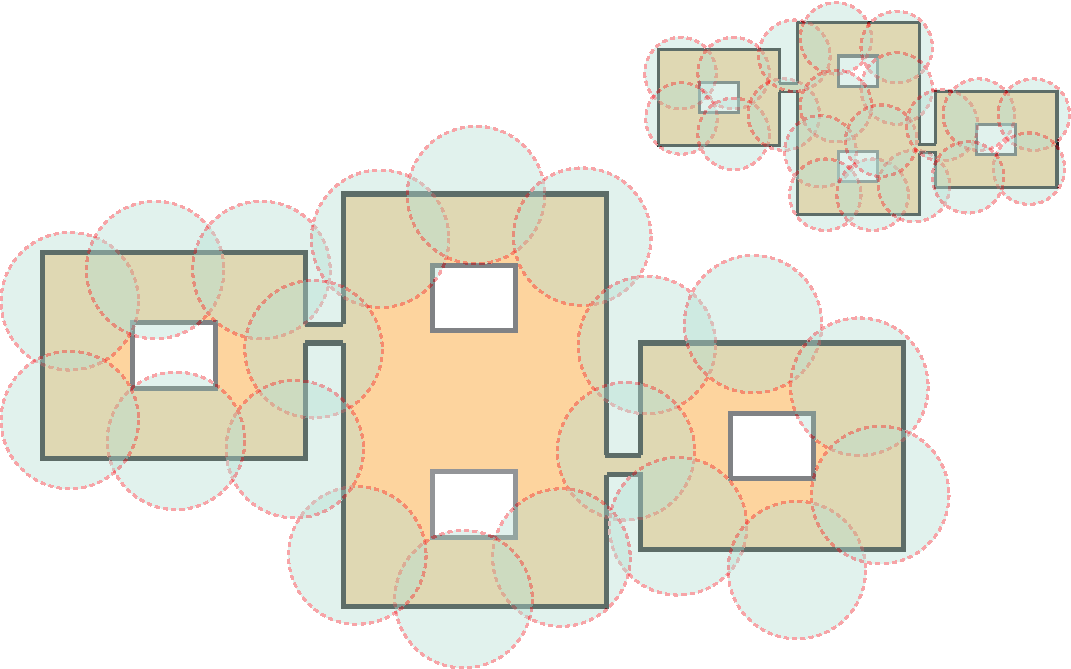
\includegraphics[width=\columnwidth]{chapters/osg/figures/example-0-eps-converted-to.pdf}
		\vspace*{1mm}
    \caption{An illustration of the \osgt setup and sample solutions.
		[center] The background shows the footprint of a building, e.g., an 
		apartment  complex. Scenarios may arise that a dangerous criminal 
		might be hiding in the building and we would like to closely monitor 
		the outer boundary of the building.	For the setting, the shaded 
		discs provide a	near-optimal cover with minimum radii for $20$ 
		mobile sensors that fully encloses the outer perimeter, computed 
		using algorithms presented in this work with optimality guarantees. 
		[upper right] A near-optimal solution for guarding the interior of
		the building footprint minus the four holes.}
    \label{fig:example0}
\end{figure}
As a summary of the study, on the side of computational complexity, we 
establish that \opgt is hard to approximate within a factor of 
$1.152$
even when the perimeter is a simple closed polygonal chain whose length
is bounded by the input size, through a reduction from 
vertex cover on planar bridgeless $3$-regular graphs.
%
A unique property of our reduction is that it shows the inapproximability gap
remains when each sensor can cover at most two disjoint perimeter 
segments. 
%
The proof also shows that \orgt is at least as hard to approximate. 
Therefore, no polynomial time algorithm may exist that solves \osgt to 
better than the $1.152$-optimal lower bound, unless P$\,=\,$NP. 
%
On the algorithmic side, we begin by providing an efficient $(1+\varepsilon)$
approximation algorithm
for a specific class of \opgt problems in which each mobile 
sensor must cover a continuous perimeter segment. This implies that the 
aforementioned inapproximability result on \opgt under the 
two-disjoint-segment sensing model is tight. 
%
For the general \osgt problem, we first describe a polynomial time 
$(2+\varepsilon)$ approximation algorithm as a reasonable approximability 
upper bound. 
%
Then, an integer linear programming (ILP) model is devised that allows 
the fast computation of highly optimal solutions for fairly large 
problem instances. 
%\jy{Maybe an example here on the scale of problems that we can solve and how fast.}
%
Results described in this paragraph, together with the introduction 
of \osgt as a practical multi-robot deployment problem focusing on global 
optimality, constitute the main contributions of this work. 

As an intermediate result toward showing the hardness of the simple polygon
coverage problem, we also supply a hardness proof of vertex cover 
on planar bridgeless\footnote{That is, the deletion of any edge does not disconnect 
the graph.} $3$-regular graphs, which may be of independent interest. 

\textbf{Related work}. Our work on optimal perimeter and region guarding 
draws inspiration from a long line of multi-robot coverage planning and 
control research, e.g., \cite{cortes2004coverage,martinez2007motion,
schwager2009optimal,pavone2009equitable,schwager2009decentralized,
pierson2017adapting}. 
%
In an influential body of work on coverage control \cite{cortes2004coverage,
martinez2007motion}, a gradient based iterative method is shown to drive 
one or multiple mobile sensors to a locally optimal configuration with 
convergence guarantees. 
%
Whereas \cite{cortes2004coverage,martinez2007motion} assume that the 
distribution of sensory information is available {\em a priori}, it is 
shown that such information can be effectively learned 
\cite{schwager2009decentralized}. 
%
Subsequently, the control method is further extended to allow the 
coverage of non-convex and disjoint 2D domains \cite{schwager2009optimal} 
and to work for mobile robots with varying sensing or actuation capabilities
\cite{pierson2017adapting}. 
%
In contrast to these control-based approaches, which produce iterative 
locally optimal solutions, \osgt emphasizes the direct computation of 
globally optimal deployment solutions and supports arbitrarily shaped
bounded (1D) perimeters and (2D) regions.

Recently, the problems of globally optimally covering perimeters using 
one-dimensional sensors have been studied in much detail 
\cite{FenHanGaoYuRSS19,FenYu2020RAL}. It is shown that when the sensors 
are homogeneous, the optimal deployment of sensors can be computed 
very efficiently, even for highly complex perimeters \cite{FenHanGaoYuRSS19}.
On the other hand, the problem becomes immediately intractable, sometimes
strongly NP-hard, when sensors are heterogeneous \cite{FenYu2020RAL}. 
Our research is distinct from \cite{FenHanGaoYuRSS19,FenYu2020RAL} in that 
we employ a (two-dimensional) range sensing model and work on the coverage 
of both perimeters and regions, which has much broader applicability. 

As pointed out in \cite{cortes2004coverage,schwager2009decentralized}, 
distributed sensor coverage, as well as \osgt, has roots in the study 
of the facility location optimization problem 
\cite{weber1929theory,drezner1995facility}, which examines the selection 
of facility (e.g., warehouses) locations that minimize the cost of delivery 
of supplies to spatially distributed customers. In theoretical computer 
science and operations research, these are known as the $k$-center, 
$k$-means, and $k$-median clustering problems \cite{har2011geometric}, 
the differences among which are induced by the cost structure. Our 
investigation of \osgt benefits from the vast literature on 
the study of $k$-center clustering and related problems, e.g., 
\cite{feder1988optimal,hochbaum1985best,gonzalez1985clustering,daskin2000new,shamos1975closest}.
%
These clustering problems are in turn related to packing 
\cite{hales2005proof}, tiling \cite{thue1910dichteste}, and the 
well-studied art gallery problems \cite{o1987art,shermer1992recent}.

\textbf{Organization}. The rest of the paper is organized as follows. 
In Section~\ref{sec:problem}, we introduce the \osgt formulation. 
Section~\ref{sec:complexity} is devoted to establishing that \osgt is 
hard to approximate to better than $1.152$-optimal, providing a theoretical
lower bound. In Section~\ref{sec:algo}, focusing on the upper bound, 
we describe algorithms that for \osgt and the special \opgt variant 
where a sensor is allowed to cover a continuous perimeter segment.
In Section~\ref{sec:expr}, we benchmark the algorithms and illustrate two 
potential applications. We discuss and conclude the work in Section~\ref{sec:conc}.



